\section{Experiment}
\label{sec:experiment}
\shuqing{Many parts in this section are much more likely to lie in implementation, introducing how \tool works. Doesn't look like experiment.}

%\shuqing{Experiment for devices and case study needed.}
To evaluate the effectiveness of \tool in different modes, we conducted three experiments on \tool using devices with USB Type-C capabilities from different OEMs, including a mobile phone, a tablet and a laptop.

\textit{Setup.} As mentioned in Section~\ref{sec:badusb}, our \tool only requires common components that are easily accessible online or in any electronic store. Here we choose the following parts to build a prototype. To begin with, we choose the Raspberry Pi 4B as the embedded computer inside \tool, which is powerful enough to process video data and has onboard WiFi chip. As for the HID emulator, we decide to use a ATMEGA32U4 board with USB protocol support. This Atmel chip is able to emulate most HID devices with our modified firmware. About the USB 3.x hub, we uses one from the Yamazawa, which supports HDMI, USB 2.0, and many other exported peripheral. Apart from these essential parts, we also uses an auxiliary power-bank to provide power for the Raspberry Pi and the mobile devices used by the victim. The image of our prototype \tool can be found in Figure~\ref{fig:armory}.

\begin{figure}[t]
	\centering
	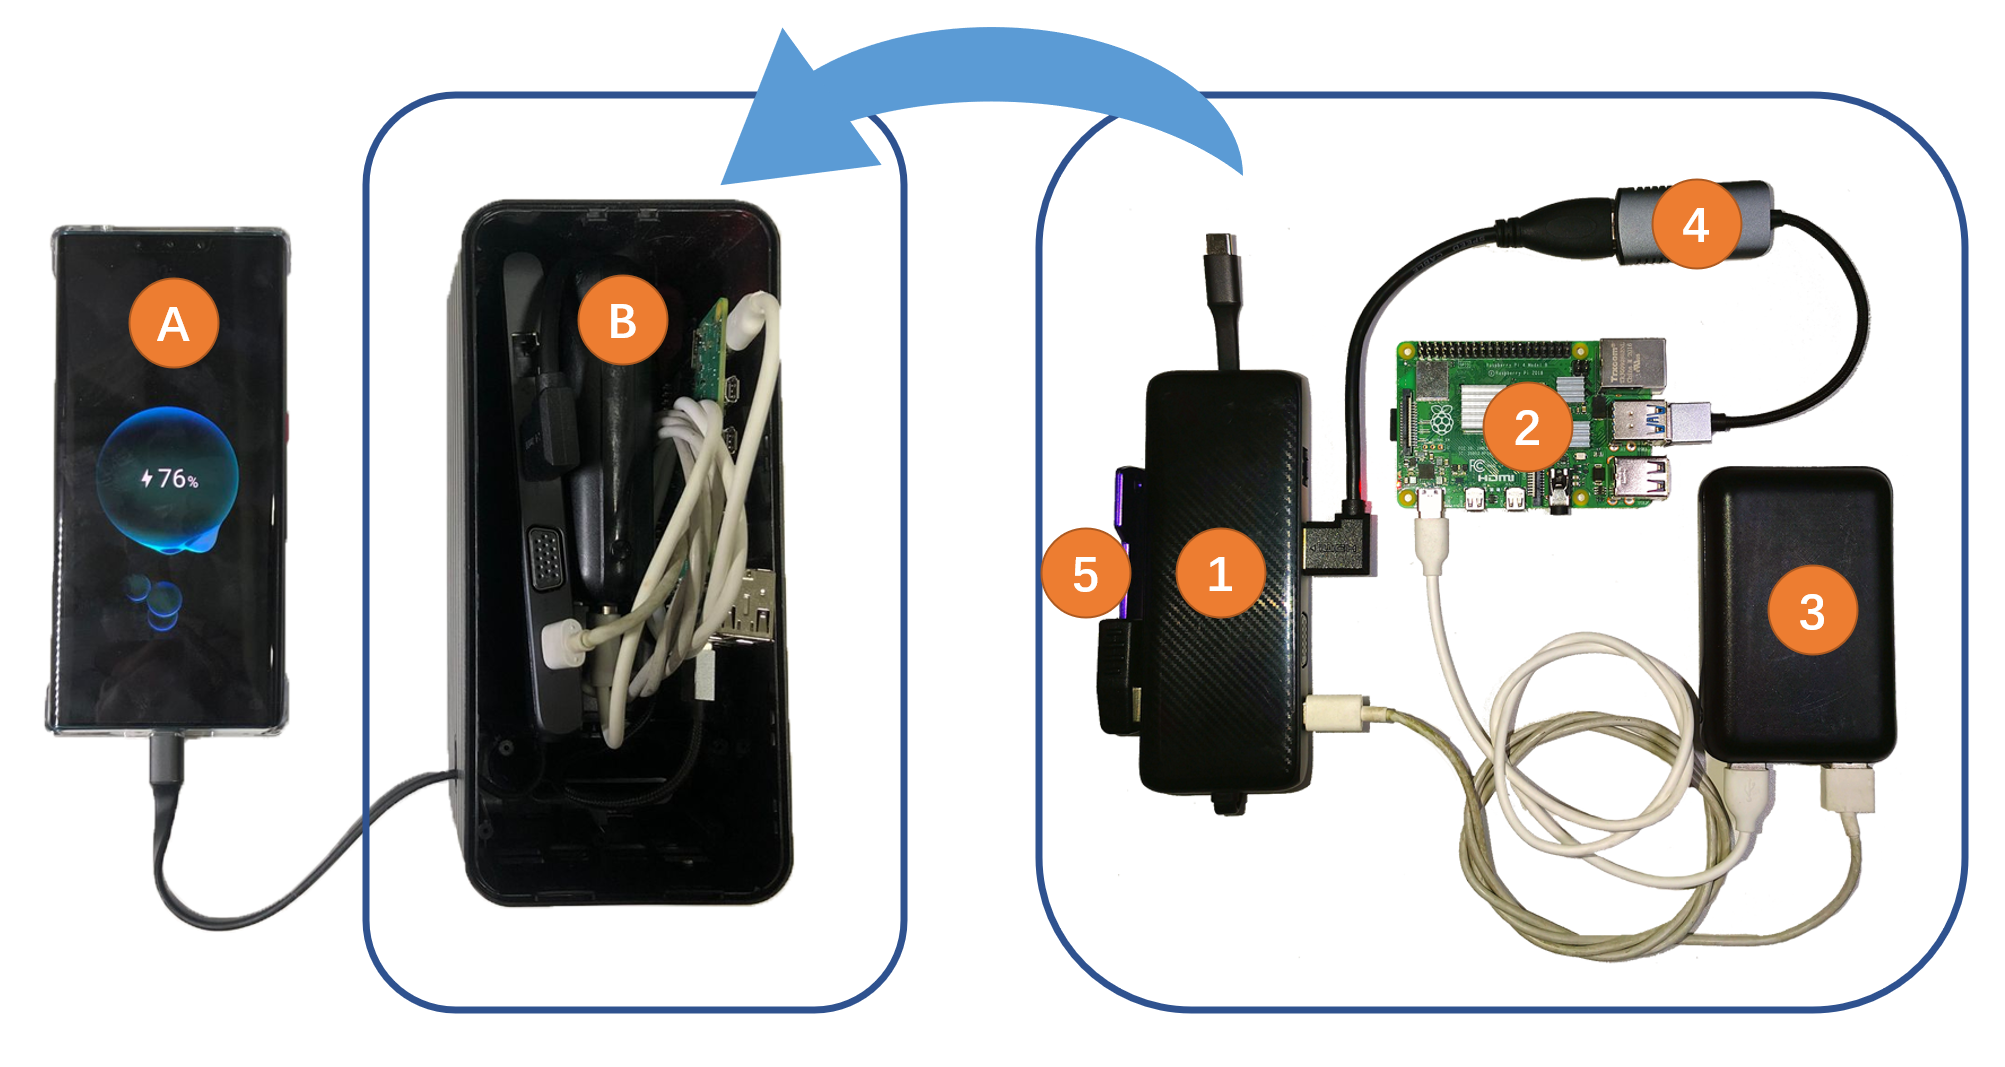
\includegraphics[width=.98\linewidth]{./Figs/armory_all.png}
	\caption{\tool}
	\label{fig:PBS_products}
\end{figure}
\subsection{Scripting mode}
In the experiment of scripting mode, we used \textit{Lenovo Xiaoxin Pro 13 2020}, a PC in Windows 10/Ubuntu OS with two USB Type-C interfaces as target device.
During this experiment, \tool disguised itself as a normal keyboard and a home-brewed version of GoodUSB\cite{tian2015defending} is deployed to test the defense bypassing. We have tried to deploy the original GoodUSB on the target device, but as the GoodUSB is proposed in 2015 and the code is too outdated to run at modern OS. We have to home-brew a similar defense mechanism according to its paper.
At the beginning, our home-brewed version of GoodUSB asked victim to manually complete a CAPTCHA to  authorize the new USB device, a.k.a our \tool. But at this time, by the design of GoodUSB, our \tool can already perform limited keystroke to complete the CAPTCHA and will be rejected only after the failure of authorization. With the video feedback from \tool, the attacker successfully completes the CAPTCHA.
Up to this point, the bypass of defense like GoodUSB is completed as our \tool already gain full function from the GoodUSB and become a trusted device. Then, our \tool works similar to the original BadUSB, inserting keystroke to perform arbitrary execution on the laptop. We tested three scripts, ranging from reverse shell backdoor to malware payload execution, all of which resulting in success.

With this experiment, we have proven the defense bypassing is possible using \tool. This also warned us that we need more thorough defense against such BadUSB attack.

\subsection{Remote control mode}
To test the capability of remote control mode, we chose \textit{iPad Pro (3rd generation)}, a tablet in iOS 14.3 with a USB Type-C interface, as the target device in this experiment.
Besides disguising as normal HID devices like a conventional BadUSB~\cite{badusb}, \tool also transmitted real-time video stream from the target device to the attacker via WiFi.
After the connection establishment, attacker performed a series actions to test the capability of \tool. At the beginning, attacker accessed album application on the iPad and obtained all the photos inside. After that, attacker tried to send messages via victim's account. At last, attacker performed a small amount of transaction using the financial application. All of these tests resulted in success and proved that \tool is a powerful attack tool.

Through this experiment, we have found that with video transmission and mouse emulation, \tool extensively expanded the attack surface of BadUSB attack, especially in mobile devices. We have archived complete hijack of victim's device in this experiment.

\subsection{Privacy extraction mode}
During the experiment of privacy extraction, we chose \textit{HUAWEI P30}, a smartphone in EMUI 9.1 (Android 9.0 based) with a USB Type-C interface, as the target device.
In privacy extraction mode, \tool passively captured video from the victim's device and used \textit{OpenCV} to identify valuable information from video stream.
When the victim viewed text or photos with text, \tool used the techniques of optical character recognition (OCR) to extract text from corresponding video frames.
In this experiment, attacker had successfully extracted text like name, address, ID number and other valuable personal information. We also tested the payment code extractor, which enables attacker to identify payment code in the video stream and perform transaction without password. As this is also a part of our case study, more details about the data extracted can be found in Section~\ref{subsec:case_study} and Table~\ref{table:information_extracted}.

After the experiment, we have found that as privacy extraction mode only passively process victim's video stream, this is a more power-efficient mode than remote control mode.

\subsection{Case study}
\label{subsec:case_study}
\subsubsection{Background}
We first introduce the technical background of our case study, sharing power bank service and QR code payment.

\textbf{Sharing Power Bank}.
Sharing power bank provides users with short-term rental of power banks.
The company deploys power bank stations in the city and users can rent a power bank from any of the power bank station, charge their device on the trip, return the rented power bank to the near station and pay the rent fee.

For an example, Brick is such a power bank sharing service provider from Sweden. It provides power bank rental service all over the Sweden and is planning on expanding their service around Europe. What's more, this service is even more popular in China, there are these stations being deployed in almost every market, store and even newsstand. This suggests that this service is becoming more and more common around the global, especially in China and Europe.
\shuqing{I think we should paraphrase instead of using the descriptions on the website directly. Just to explain \textbf{what we need}.}

\begin{figure}[t]
	\centering
	\includegraphics[width=.4 \linewidth]{./Figs/Brick_station.png}
	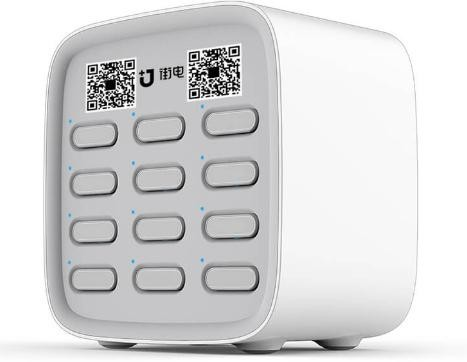
\includegraphics[width=.4 \linewidth]{./Figs/jiedian.jpg}
	\caption{Two power banks station products}\shuqing{Photos that we took.}
	\label{fig:PBS_products}
\end{figure}

\yechang{add hyperlink or reference to Brick's website or Brick App on App Store/Google Play.}

\yechang{Add more examples of power bank sharing to show that it is widely used?}
\shuqing{May use statistics (instead of concrete examples) to explain it.}

Not only does sharing power bank provides convenience to users, but it also brings security issues. 
We noticed that most of the power bank stations do not check the integrity of power banks during the rental process, and users are hardly cautious to check the power banks when connecting their devices. 
An attacker are able to modify his/her rented power banks and return it to a power bank station causing potential threat to subsequent users.


\textbf{QR Code Payment}.
QR code payment is a new type of payment method that are popular in China. Its most well known cases are WeChat Pay and Alipay. QR code payment provides merchant and client a convenient way of offline payment while ensuring equivalent security as the credit card. This explains why it becoming widely used in China.
QR code payment is typically performed in the following steps:
\ding{182} The client presents payment QR code on mobile device to the merchant.
The QR code is encoded with a globally unique ID to identify the client's account.
\ding{183} The merchant scans the payment QR code and charges corresponding amount of money.
By presenting this QR code, the client authorizes proceeding charge.
\ding{184} An transaction generated by this scan is sent to the payment service provider.
Then the payment service provider requests the client to confirm the transaction.
\ding{185} After confirmation, the payment service provider proceed with this transaction and return the payment result to both the merchant and the client.
\shuqing{I think this paragraph can be shorter. No need to explain so many details.}
\hongyi{Dont know how to be more concise.}

\begin{figure}[t]
	\centering
	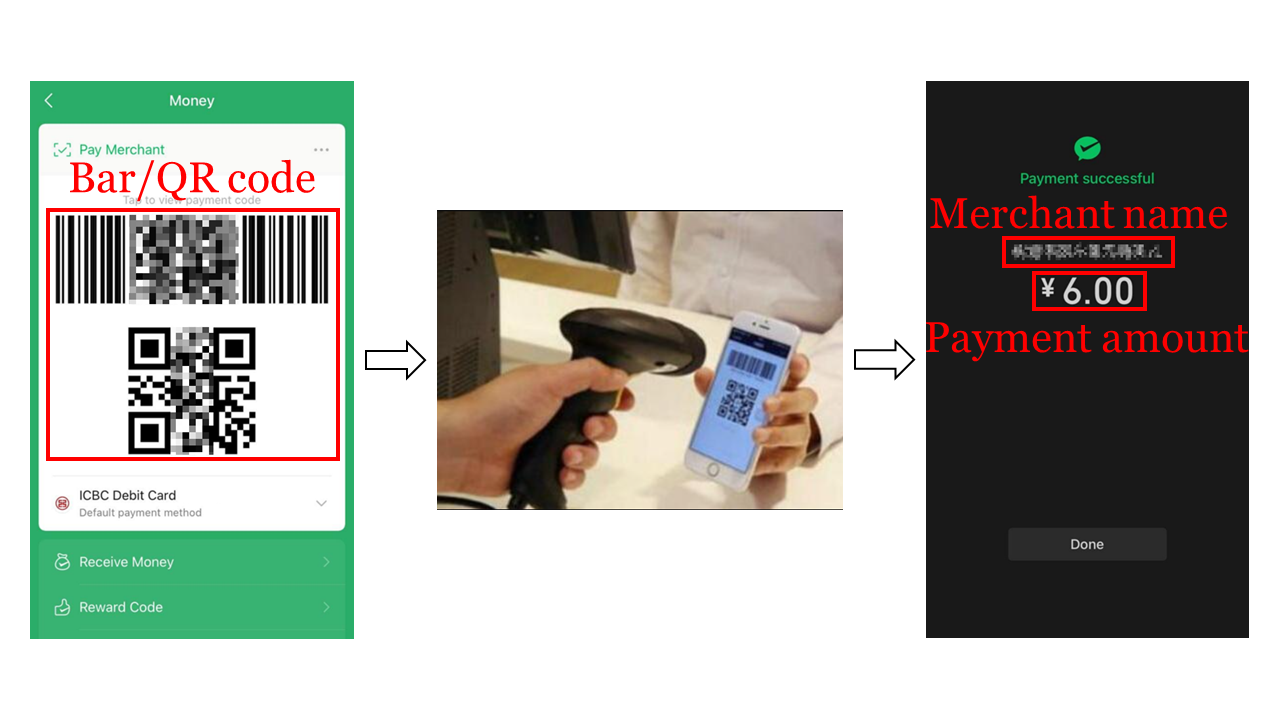
\includegraphics[width=\linewidth]{./Figs/qr_code_payment.png}
	\caption{Bar/QR code payment procedure}
	\label{fig:qr_payment_procedure}
\end{figure}


In the real-world scenario, some payment service providers provide special rules for micropayment purchases.
A micropayment is pre-determined by the payment service provider with thresholds in the user agreement.
For example, WeChat Pay~\cite{Wechat-pay} regards transaction under USD \textdollar 154 as micropayments.
Different from a typical payment procedure, when micropayments are made, confirmations can be applied automatically without clients' permission which aims to provide convenience to both merchant and client.
If a victim's payment code is leaked to the attackers, they can use the that code to authorize multiple micropayments without permission.
In order to prevent such cases, both Alipay and WeChat Pay has designed a refreshing mechanism for the payment code, which is to refresh the QR code every minute. This is sufficient to stop attack like sneak shots, but unable to stop real-time attack like our \tool.
In summary, the payment QR code is highly sensitive on users' devices and our following case study is about how to obtain this code using modified power bank, our \tool.

\subsubsection{Attack Scenario}
In this part, we will introduce a real life attack scenario to prove that our \tool is a practical offensive tool.
This scenario can be decomposed into the following steps.
\begin{enumerate}[I. ]
	\item The attacker rents a power bank from one of power bank stations and replace the internal components with our \tool.
	\item After the modification, \tool is returned to another power bank station in a crowded area like airport or railway station, which increases the probability of success.
	\item Other users borrows the modified power bank and connects it to their own devices, becoming the victim of \tool.
	\item The attacker now has complete control over victim and can perform various attack using different modes.
\end{enumerate}
Here we summarizes the possible threats toward user under different modes. \hongyi{Better way to express this?}
First, under scripting mode, the attacker is able to implant malware and backdoor script into victims' devices. Moreover, using privacy extraction mode, once the victims access their private data like QR payment  code or album, their private data will be immediately transmitted via \tool to the attacker. Lastly, with remote control mode, the attacker has complete control over the victims' device and can do anything they want.

\shuqing{Background is longer than real user study.}
As the functionality and effectiveness of scripting mode and remote control mode is rather clear, the former works similar to original BadUSB, the latter hijacks the victim's device completely.\hongyi{I dont know if it's a good enough reason}
Here we only validate the usability of privacy extraction mode and conducted a user study.
\shuqing{10 volunteers.}
We invited 6 volunteers to participate, who are unconscious of \tool details.
Before the experiment, we disclose to the volunteers about how their data might be used and request permission from both the volunteers and the institutional ethics review boards.
During the experiment, volunteers took turns to use their phones for half an hour with \tool connected, which are considered as a normal power bank.
In order to obtain data close to real life, they are requested to use phones just like when they use the shared power bank outside.
After the experiment, we introduced to them about our attack, analyze the screen recordings together to make sure their personal data is not at risk.
\shuqing{Do we need to mention that agreement the conference required here?}
\hongyi{I'm also quite concern about this.}


\subsubsection{Result}
After collecting the videos, we analyzed the video both automatically and manually.
During the automatic analysis, we used scripts to perform OCR recognition for each frame in the recorded video and stored all of the OCR results in a database.
At last, there are 38329 pieces of data collected among 6 volunteers.
\shuqing{The data may need to be updated.}
With these results, we could learn what content the victim was browsing.
Additionally, some keywords such as \textit{account, username and password} often appear with users' input data because they are often used as labels of input boxes.
Such keywords are more likely to lead us to user-specific data.
For example, when we searched with \textit{account} as keyword, victim's accounts can be found in the database, as shown in the Table~\ref{tab:ocr_keyword_example}.
\shuqing{Statistics.}
The frame number is the position of this frame in the recorded video, which indicates a target for manual analysis for further data extraction.

\begin{table*}[t]
	\centering
	\begin{tabular}{|l|l|l|l|}
		\hline
		Keyword  & Text                                                                                                                          & Name                           & Frame Number \\ \hline
		username & X 8B cas.******.edu.cn Username: 117***18 Password:                                                                           & \textless{}user1\textgreater{} & 385          \\ \hline
		username & Login Weibo Login with SMS and verification code ...... +86 151****4587 & \textless{}user5\textgreater{} & 1947         \\ \hline
		username & QQ 14*****50| Login with phone number New user registration 2345678 9 0                                                       & \textless{}user3\textgreater{} & 4308         \\ \hline
		username & connect to *** username h*****l Save account information Open VPN.....                                                        & \textless{}user6\textgreater{} & 7925         \\ \hline
		+86      & Login with phone number ...... +86 186****2483 |                                                                              & \textless{}user1\textgreater{} & 313          \\ \hline
	\end{tabular}
	\caption{Example of searching OCR results with some keywords}
	\label{tab:ocr_keyword_example}
\end{table*}


In the manual analysis, we replayed the recorded video and extracted sensitive information.
The data we collected are listed in the Table~\ref{table:information_extracted}.
Accounts of internet applications such as Apple, iCloud, Facebook, Twitter, etc. can be obtained.
Moreover, all of the typing inputs on the virtual keyboard, including the system keyboard and the built-in security keyboard of the financial applications, can be clearly recorded.
We can obtain the plain text of password such as WiFi password.
Furthermore, the received SMS verification code (usually used to confirm real-name authentication) can be obtained when it appears in the top notification bar.

In summary, though we can't directly obtain the user's password on the lock screen, we can still check all of the information presented on the screen, extract private information including but not limited to social accounts, bank accounts, personal financial situation, etc., if the user unconsciously unlocks the screen.
It is worth mentioning that, those \textit{secure keyboards} built in some financial apps just disrupt keyboard sequences, they can't prevent attacks similar as \tool.

\begin{table*}[t]
	\centering
	\begin{tabular}{|c|c|c|c|c|}
		\hline
		Application Column  & Application & Private information leaked                       \\
		\hline
		Finance App         & Alipay      & Alipay account, personal assets(blance)          \\
		\hline
		Social  Finance App & WeChat      & WeChat account, blance, chat history             \\
		\hline
		Social App          & QQ          & QQ account, interpersonal nexus, chat history    \\
		\hline
		Social App          & Twitter     & Twitter account, interpersonal nexus             \\
		\hline
		Social App          & Gmail       & Gmail account, mail records                      \\
		\hline
		Finance App         & ICBC        & ICBC account, password, personal assets(blance)  \\
		\hline
		Finance App         & Paypal      & Paypal account, blance, bank accounts            \\
		\hline
		Tool                & Chrome      & Sites visited                                    \\
		\hline
		Tool                & Health      & personal physical metrics      					 \\
		\hline
	\end{tabular}
	\linebreak
	\caption{Information extracted}\shuqing{Compress.}
	\label{table:information_extracted}
\end{table*}
